\documentclass[main.tex]{subfiles}

\usemintedstyle{bw}

\begin{document}

\renewcommand\stamppartname{Копії графічних матеріалів}
%\renewcommand\lastpagelabel{PartLastPageapp}
\newpart{appendixa}{ІАЛЦ.467100.004 Д1}

\begin{specialpage}
  \MakeUppercase{Додаток А}\\
  \MakeUppercase{\stampname{}}

  \vspace*{\fill}
  \textbf{\MakeUppercase{\stamppartname{}}}\\
  Аркушів 7%\pageref{\lastpagelabel{}}

  \vspace*{\fill}
  \mypagefooter{}
\end{specialpage}

\newappendix{appI}{ІАЛЦ.467100.004 Д1}{\appendixI{}}
\begin{center}
\noindent%\includegraphics[width=\textwidth]{1}
\begin{minted}[breaklines,fontsize=\footnotesize]{ebnf}
comment = '/', '/', {all characters - '\n'};

all characters = ? all unicode characters ?;

id = (alpha | "_"), {alpha | "_" | digit};

alpha = ? all latin letters ?;
digit = "0" | "1" | "2" | "3" | "4" | "5" | "6" | "7" | "8" | "9";

number = number value, [number type specifier];

number value = hexadecimal number
  | binary number
  | decimal number;

hexadecimal number = '0x', hex digit, {hex digit};
binary number = '0b', binary digit, {binary digit};
decimal number = digit, {digit};

hex digit = digit |
  'A' | 'B' | 'C' | 'D' | 'E' | 'F' |
  'a' | 'b' | 'c' | 'd' | 'e' | 'f';

binary digit = '0' | '1';

number type specifier =
  'u8' | 'u16' | 'u32' | 'u64' |
  'i8' | 'i16' | 'i32' | 'i64';

string = '"', {all characters - '\n' - '\\' | '\\', escaped symbol}, '"';

escaped symbol = 'n' | 'r' | 't' | '\\' | "'" | '"'
  | 'x', hexadecimal digit, hexadecimal digit;

struct definition = ['pub'], 'struct', id,
  '{', {field definition}, '}';

field definition = ['pub'], id, ':', type, ';';

enum definition = ['pub'], 'enum', id,
  '{', enum options, '}';

enum options = [option, [',', enum options], [',']];

option = id, ['=', expression];

function def = ['pub'], id, '(', args, ')', ':', type,
  compound statement;

args = [argument, [',', args]];

argument = id, ':', type;

impl block = 'impl', [type, 'for'], type,
  '{', {function def}, '}';

trait def = 'trait', type, [':', type],
  '{', {function def | function decl}, '}';

function decl = ['pub'], id, '(', args, ')', ':', type;

type placeholder = '_', {alpha | digit};

conditional expr =
  'if', expression, compound statement,
  ['else', (conditional expr | compound statement)];
\end{minted}
\end{center}

\newappendix{appII}{ІАЛЦ.467100.005 Д2}{\appendixII}
\begin{center}
% @startuml
%
% class Module
% class Import
% class ImportRename
% class Decl
% class Attribute
% class FieldDecl
% class Scope
% class TypeParam
% class Param
% class Type
% class Expr
% class Mutability
% class Literal
%
% Module *-- "many" Import
% Module *-- "many" Decl
%
% Import *-- "many" ImportRename
%
% Decl *-- Scope
% Decl *-- "many" TypeParam
% Decl *-- "many" Parm
% Decl *-- Type
% Decl *-- Expr
% Decl *-- FieldDecl
% Decl *-- Attribute
%
% Attribute *-- Expr
%
% FieldDecl *-- Scope
% FieldDecl *-- Id
% FieldDecl *-- Type
%
% TypeParam *-- Id
%
% Param *-- Id
% Param *-- Type
%
% Type *-- "many" Type
% Type *-- Id
% Type *-- Mutability
%
% Expr *-- Literal
% Expr *-- QualifiedName
% Expr *-- Expr
%
% Statement *-- Expr
% Statement *-- Id
%
% @enduml
\noindent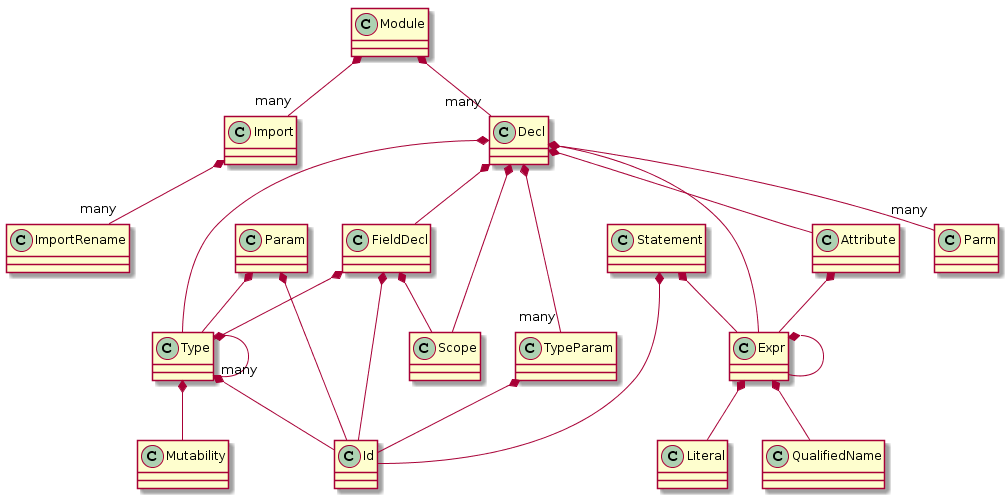
\includegraphics[width=\textheight-25mm,angle=90,origin=c]{master_ast}
\end{center}


\newappendix{appIII}{ІАЛЦ.467100.006 Д3}{\appendixIII}
\begin{center}
\noindent%\includegraphics[width=\textwidth]{3}
\begin{equation}
  \tag*{(E-App1)}
  \frac{t_1 \rightarrow t_1'}{t_1 t_2 \rightarrow t_1' t_2}
\end{equation}

\begin{equation}
  \tag*{(E-App2)}
  \frac{t_2 \rightarrow t_2'}{v_1 t_2 \rightarrow v_1 t_2'}
\end{equation}

\begin{equation}
  \tag*{(E-TApp)}
  \frac{t_1 \rightarrow t_1'}{t_1 [T_2] \rightarrow t_1' [T_2]}
\end{equation}

\begin{equation}
  \tag*{(E-TAppTAbs)}
  (\lambda X <: T_{11} . t_{12}) [T_2] \rightarrow [X \mapsto T_2]t_{12}
\end{equation}

\begin{equation}
  \tag*{(E-AppAbs)}
  (\lambda x : T_{11} . t_{12}) v_2 \rightarrow [x \mapsto v_2]t_{12}
\end{equation}

\end{center}


\newappendix{appIV}{ІАЛЦ.467100.007 Д4}{\appendixIV}
\begin{center}
\noindent
  \begin{equation}
    \tag*{(T-Var)}
    \frac{x : \sigma \in \Gamma}{\Gamma \vdash x : \sigma}
  \end{equation}
  \begin{equation}
    \tag*{(T-App)}
    \frac{\Gamma \vdash e_1 : \tau_1 \rightarrow \tau_2 \quad \Gamma \vdash e_2 : \tau_1}{\Gamma \vdash e_1 e_2 : \tau_2}
  \end{equation}
  \begin{equation}
    \tag*{(T-Lam)}
    \frac{\Gamma, x : \tau_1 \vdash e : \tau_2}{\Gamma \vdash \lambda x . e : \tau_1 \rightarrow \tau_2}
  \end{equation}
  \begin{equation}
    \tag*{(T-Let)}
    \frac{\Gamma \vdash e_1 : \sigma \quad \Gamma, x : \sigma \vdash e_2 : \tau}{\Gamma \vdash \text{let} \, x = e_1 \, \text{in} \, e_2 : \tau}
  \end{equation}
  \begin{equation}
    \tag*{(T-Gen)}
    \frac{\Gamma \vdash e : \sigma \quad \overline{\alpha} \notin \textbf{ftv}(\Gamma)}{\Gamma \vdash e : \forall \, \overline{\alpha} \; . \; \sigma}
  \end{equation}
  \begin{equation}
    \tag*{(T-Inst)}
    \frac{\Gamma \vdash e : \sigma \quad \sigma_1 \sqsubseteq \sigma_2}{\Gamma \vdash e : \sigma_2}
  \end{equation}
\end{center}


\newappendix{appV}{ІАЛЦ.467100.008 Д5}{\appendixV}
\begin{center}
\noindent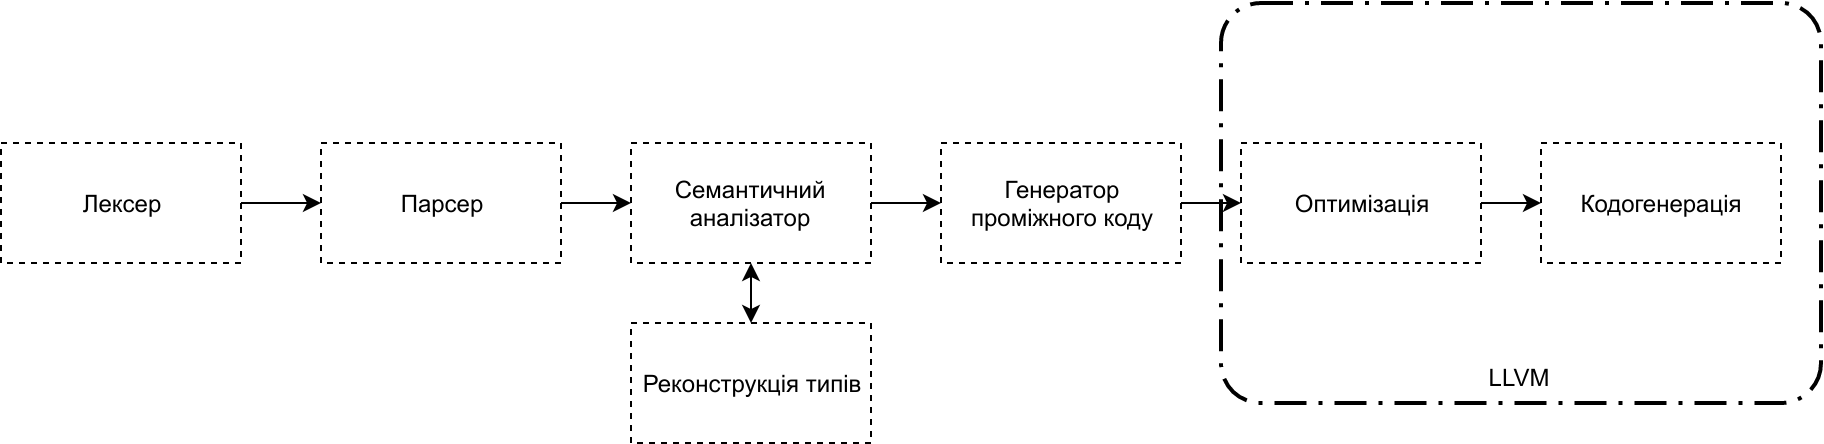
\includegraphics[width=\textheight-25mm,angle=90,origin=c]{functional}
\end{center}


\newappendix{appVI}{ІАЛЦ.467100.009 Д6}{\appendixVI}
\begin{center}
\noindent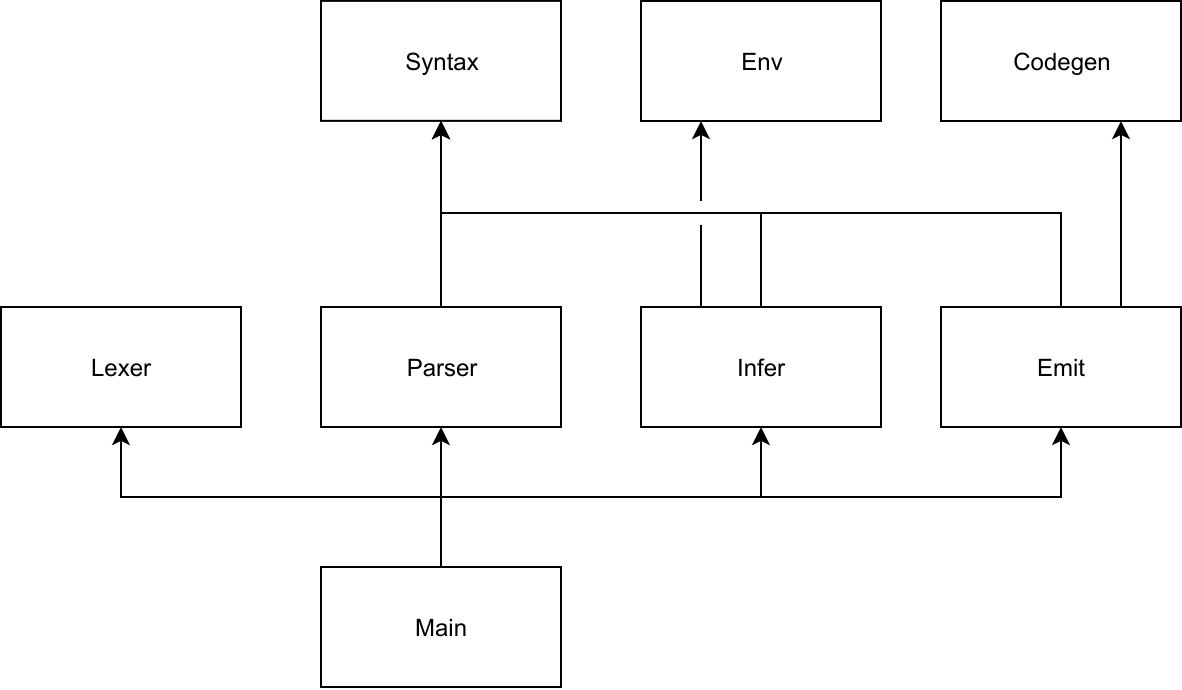
\includegraphics[width=\textheight-25mm,angle=90,origin=c]{components}
\end{center}

\end{document}
